% !TeX root = ../main.tex
\section{Capteur thermistance (SEMI833-ET)}

\subsection{Mesure manuelle de la température ambiante}
\label{subsec:ntc_ambiante}

La thermistance CTN (SEMI833-ET) présente une résistance nominale de \qty{103.6}{\kilo\ohm} à \qty{20}{\degreeCelsius}. 
À l'aide du multimètre de table Keysight 34460A (mode 2 fils, 6½ digits), la résistance mesurée à l'air ambiant du laboratoire est $R_{\text{mes}} = \qty{97.20}{\kilo\ohm}$.

D'après la table de référence du constructeur, la sensibilité moyenne dans cet intervalle ($[20\,^\circ\text{C}\,;\,25\,^\circ\text{C}]$) vaut $p_{\text{moy}} = \frac{4.70 + 3.63}{2} = \qty{4.165}{\kilo\ohm\per\degreeCelsius}$. Comme la résistance mesurée est inférieure à la valeur à \qty{20}{\degreeCelsius}, la température ambiante est supérieure à \qty{20}{\degreeCelsius} :
\begin{equation}
    T_{\text{amb}} = 20 + \frac{R_{\text{nom, } 20^\circ\text{C}} - R_{\text{mes}}}{p_{\text{moy}}} = 20 + \frac{103.60 - 97.20}{4.165} = \mathbf{\qty{21.54 \pm 0.80}{\degreeCelsius}}
\end{equation}
L'incertitude est dominée par la tolérance de fabrication de la perle ($\pm \qty{0.8}{\degreeCelsius}$), l'incertitude du multimètre ($< \qty{0.005}{\degreeCelsius}$) étant tout à fait négligeable.

\subsection{Mesure par pont diviseur et calcul d'auto-échauffement}
\label{subsec:ntc_pont}

Le conditionnement du capteur est réalisé par un pont diviseur alimenté sous $V_{CC} = \qty{14.00}{\volt}$ avec une résistance série étalonnée $R = \qty{462.35}{\kilo\ohm}$ (valeur nominale \qty{470}{\kilo\ohm}). La relation inverse programmée sous LabVIEW pour retrouver $R_{NTC}$ à partir de la tension mesurée $U_{NTC}$ s'exprime par :
\begin{equation}
    R_{NTC} = \frac{R \cdot U_{NTC}}{V_{CC} - U_{NTC}}
    \label{eq:formule_rntc}
\end{equation}

À température ambiante ($R_{NTC} \approx \qty{97.20}{\kilo\ohm}$), la tension aux bornes de la CTN, la puissance Joule dissipée et l'auto-échauffement théorique (avec $\delta \approx \qty{0.7}{\milli\watt\per\degreeCelsius}$ en air calme) valent :
\begin{equation}
    U_{NTC} = 14.00 \cdot \frac{97.20}{462.35 + 97.20} \approx \qty{2.43}{\volt} \quad \implies \quad P = \frac{U_{NTC}^2}{R_{NTC}} \approx \qty{0.061}{\milli\watt} \quad \implies \quad \Delta T = \frac{P}{\delta} \approx \mathbf{\qty{0.09}{\degreeCelsius}}
\end{equation}
Cet échauffement de moins d'un dixième de degré reste négligeable devant la tolérance du capteur ($\pm \qty{0.8}{\degreeCelsius}$), ce qui valide le choix de la résistance série $R \approx \qty{470}{\kilo\ohm}$.

\subsection{Chaîne d'acquisition et conversion sous LabVIEW}
\label{subsec:ntc_labview}

L'acquisition est réalisée avec la carte National Instruments PCIe-6321 :
\begin{itemize}[leftmargin=1.2cm,topsep=2pt,itemsep=1pt]
    \item \textbf{Configuration différentielle :} La tension $U_{NTC}$ est mesurée en mode différentiel afin de rejeter le bruit de mode commun et les parasites de masse.
    \item \textbf{Cadencement :} Boucle cadencée à une période d'échantillonnage de \qty{20}{\milli\second} (\qty{50}{\hertz}).
    \item \textbf{Conversion en température :} Calcul de $R_{NTC}$ par l'équation~\eqref{eq:formule_rntc}, puis interpolation dans la table nominale \texttt{Echelle\_SEMI833.lvm} via le sous-VI « Scaling and Mapping ».
\end{itemize}

\subsection{Mesures en flux d'air chaud et suréchantillonnage}
\label{subsec:ntc_oversampling}

Le capteur est exposé au flux d'air chaud d'un sèche-cheveux durant environ \qty{10}{\second} selon deux modes d'acquisition :
\begin{enumerate}[leftmargin=1.2cm,topsep=2pt,itemsep=1pt]
    \item \textbf{Mode standard :} lecture échantillon par échantillon cadencée à \qty{20}{\milli\second} ($N = 520$ points) ;
    \item \textbf{Mode suréchantillonné :} moyenne arithmétique matérielle de 100 échantillons par point affiché ($N = 375$ points).
\end{enumerate}

\begin{figure}[H]
    \centering
    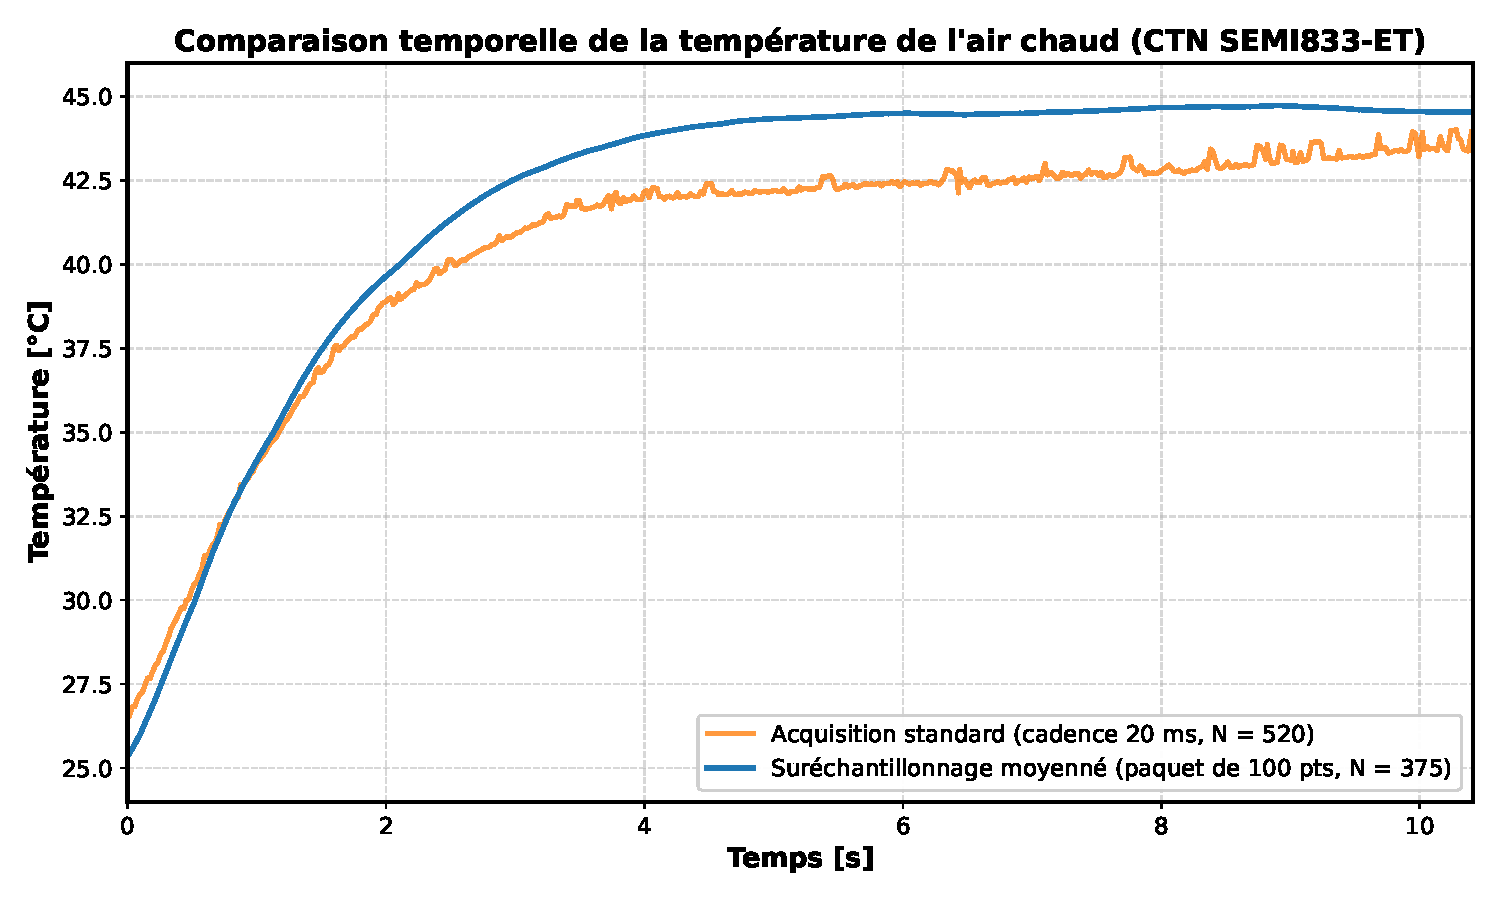
\includegraphics[width=0.72\textwidth]{assets/graphs/comparaison_ntc_oversampling.pdf}
    \caption{Comparaison temporelle de la température sous flux d'air chaud : mode standard cadencé à \qty{20}{\milli\second} et mode suréchantillonné (moyenne de 100 échantillons par point).}
    \label{fig:diff_over_normal}
\end{figure}

\subsubsection*{Analyse statistique et répétabilité expérimentale}
L'évaluation statistique sur l'ensemble de l'enregistrement et sur le palier stabilisé donne :
\begin{itemize}[leftmargin=1.2cm,topsep=2pt,itemsep=1pt]
    \item \textbf{Série standard :} globale $\bar{T} = \qty{40.56 \pm 0.17}{\degreeCelsius}$ ($\sigma = \qty{3.96}{\degreeCelsius}$), palier stabilisé $\bar{T}_{\text{stab}} = \mathbf{\qty{41.13 \pm 0.13}{\degreeCelsius}}$ ($\sigma = \qty{2.98}{\degreeCelsius}$) ;
    \item \textbf{Série suréchantillonnée :} globale $\bar{T} = \qty{41.90 \pm 0.25}{\degreeCelsius}$ ($\sigma = \qty{4.75}{\degreeCelsius}$), palier stabilisé $\bar{T}_{\text{stab}} = \mathbf{\qty{42.83 \pm 0.17}{\degreeCelsius}}$ ($\sigma = \qty{3.15}{\degreeCelsius}$).
\end{itemize}
Le suréchantillonnage atténue théoriquement le bruit électronique de conversion d'un facteur $\sqrt{100} = 10$. Néanmoins, l'écart-type mesuré en régime stabilisé reste comparable ($\sigma \approx \qty{3}{\degreeCelsius}$) : le bruit est dominé par les turbulences réelles du flux d'air chaud et non par l'ADC.

De plus, l'écart de température moyenne entre les deux essais ($\Delta \bar{T} \approx \qty{1.7}{\degreeCelsius}$) s'explique par l'absence de répétabilité de la manipulation : le sèche-cheveux et la perle étaient tenus à la main sans support fixe, provoquant de légères variations de position, de distance et d'angle dans le cône d'air chaud.
